\chapter{Assignment of Individual Frames} 
\label{app:IndFrameAss}

\paragraph{Abstract view of coordinate frames}
For a better overview, the drawing of the robot in figure \ref{fig:RefFrame} can be removed, which reveals the pure coordinate frames. In figure \ref{fig:RefFrameAbstract} is described, in which relation the coordinate frames stand to each other.

\begin{figure}[H]
	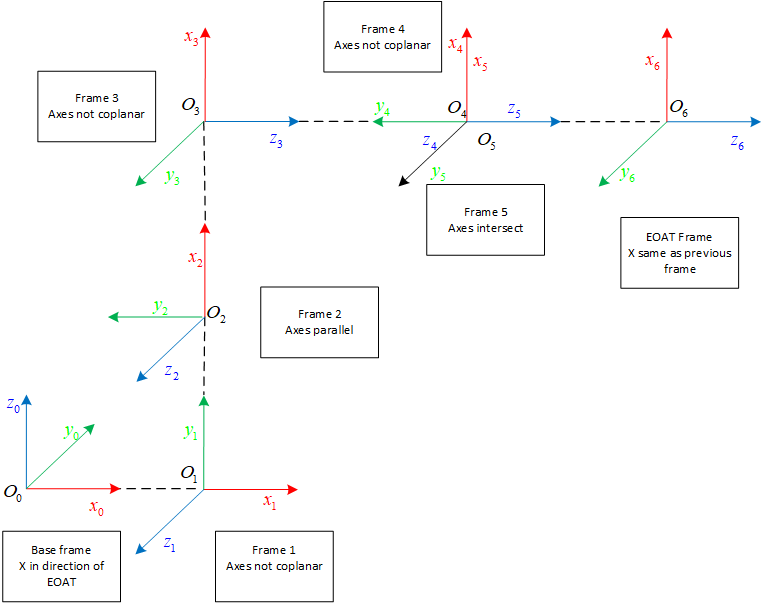
\includegraphics[
	width=1\linewidth,
	center,
	keepaspectratio,
	]{coordinateFrames/CoordinateFrames}
	\caption{Coordinate reference frames for Fanuc 210F}
	\label{fig:RefFrameAbstract}
\end{figure}

\paragraph{Steps to find individual frames}
The steps how to find each individual link-coordinate frame can be described as following:

\paragraph{Frame 0 (base)}
The frame mapping starts with the base frame. For the base frame the z-axis is given through joint $j_1$. Origin of frame 0 is put into joint 1.
The x-axis is chosen to point in direction of of the \ac{EOAT} in standard pose. For standard pose see 
\ref{fig:RefFrame}
.
This pose will also be chosen for alignment of all distal frames.
\\
This assignment of the base frame can be optimized to minimize the \ac{DH}-parameters. By moving the base frame out of the joint on the same x/y-surface as frame 1, $d_1$ can be set to zero without changing the kinematics. Simply an offset in the z-axis of the generalized world coordinates for the end effector is added.

%\begin{figure}[h]
%	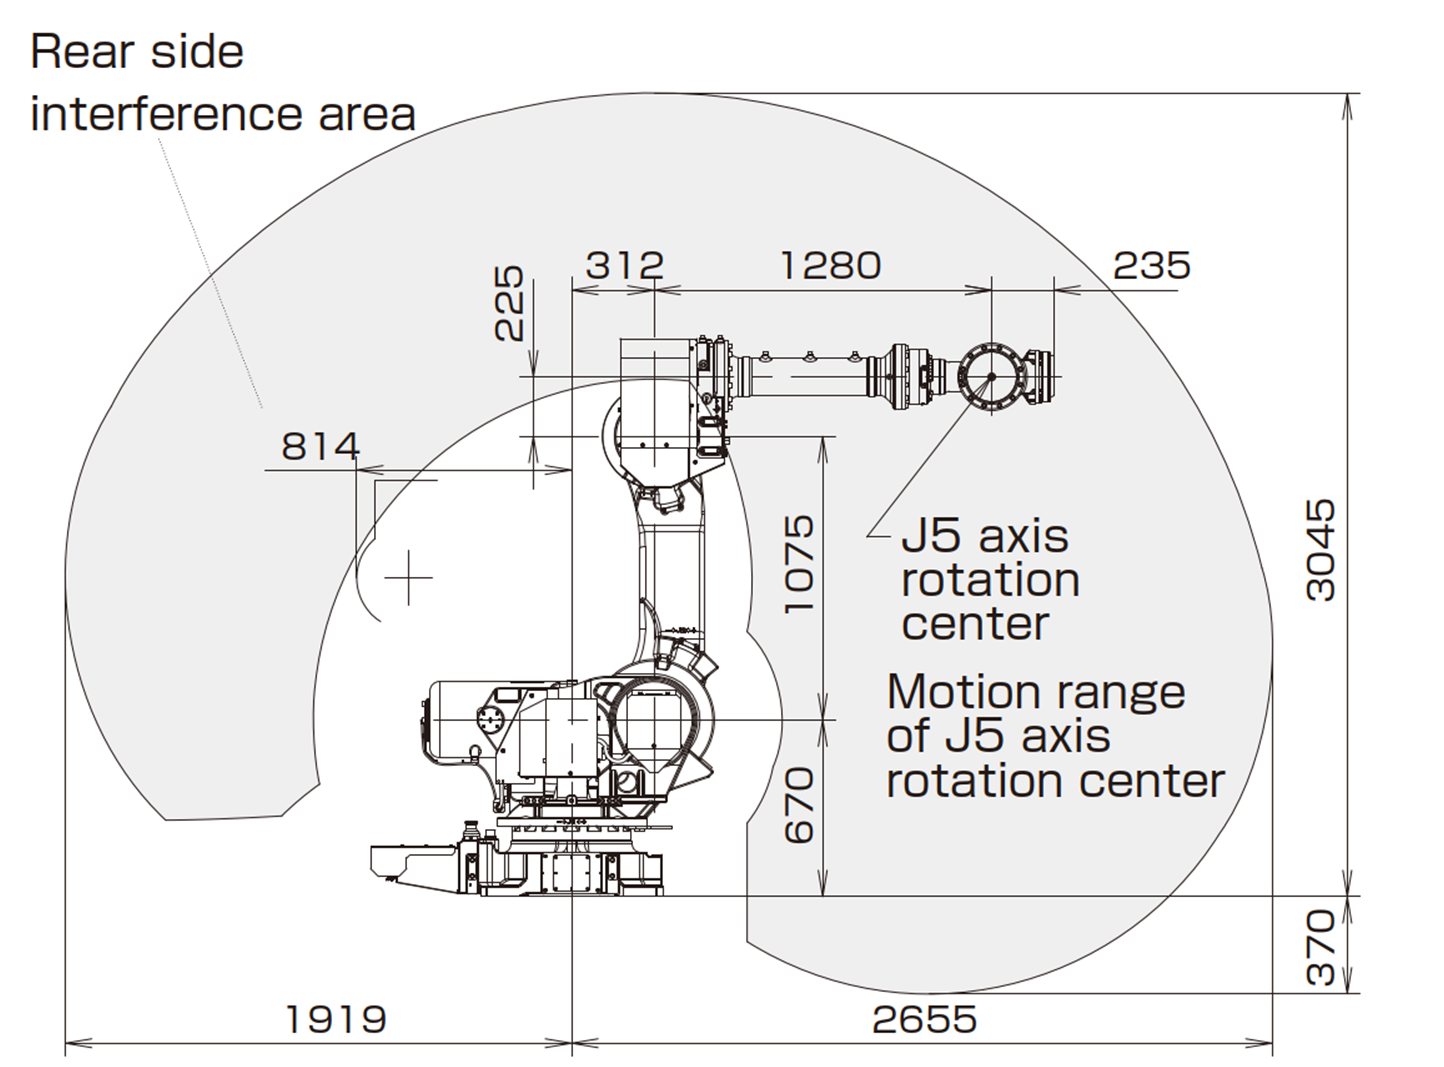
\includegraphics[
%	width=1\linewidth,
%	center,
%	keepaspectratio,
%	]{coordinateFrames/standardPose}
%	\caption{Standard pose of the robot}
%	\label{fig:StandardPose}
%\end{figure}

\paragraph{Frame 1}
For frame 1, the z-axes are not coplanar. 
Because of that, the  $z_0$-axis is extended until a common normal can be found that intersects with $z_i$ to define the origin $O_1$.
$x_1$ departs from $O_1$ along the common normal.
$y_1$ is added according to the right hand rule.

\paragraph{Frame 2}
As seen, in image \ref{fig:zi_Axes}, axes $z_2$ and $z_1$ are parallel. $O_2$ can be found at the intersection of the normal through $O_1$ with $z_2$. $x_2$ follows the common normal with joint 4.
$y_2$ is added according to the right hand rule.

\paragraph{Frame 3}
Joint 3 and joint 4 are not exactly aligned (see image \ref{fig:RefFrame}), which prevents the z-axes to intersect. That's why axes $z_3$ and $z_2$ are not coplanar. 
$z_3$ runs parallel through the link 3, due to the orientation of the rotational axis.
As the common normal between $z_3$ and $z_2$ defines $x_3$, which in turn gives $O_3$, the origin can be found far away from the physical position of the joint.
$y_3$ is added according to the right hand rule.

\paragraph{Frame 4}
Joint 5 lies in line with joint 4.
As $z_3$ follows this line, the axes  $z_4$ and $z_3$ intersect in the centre of joint 5, which gives $O_4$. 
$x_4$ leaves the plane spanned by  $z_4$ and $z_3$ perpendicular.
The positive direction of $x_4$ is chosen to be similar as in frame 3 for simplicity.
$y_4$ is added according to the right hand rule and points in direction of frame 3.

\paragraph{Frame 5}
As $z_5$ lies  in line with $O_4$, the axes  $z_5$ and $z_4$ intersect in $O_4$ which puts $O_5$ at the same position as $O_4$.
$x_5$ leaves the plane spanned by  $z_5$ and $z_4$ perpendicular.
The positive direction of $x_5$ is chosen to be similar as in frame 4 for simplicity, which puts $x_5$ and $x_4$ on top of each other. 
$y_5$ is added according to the right hand rule and as $z_5$ is turned 90 degrees relative to $z_4$ around $x_{4,5}$, $y_5$ is turned 90 degrees relative to $z_4$ around $x_{4,5}$ as well.

\paragraph{Frame 6 (EOAT)}
$z_6$ lies in line with $z_5$ and is consequently parallel.
as there are no distal joints, to reference $x_6$, it can be chosen arbitrarily. 
For simplicity, it is chosen to be similar as in frame 5. 
$y_6$ is added according to the right hand rule.\\
\\

